\chapter{Assignment-Probability}
\begin{enumerate}
	\item Consider a random walker on a square lattice. At each step the walker moves to a nearest neighbour site with equal probability for each of the four sites. The walker starts at the origin and takes 3 steps. The probability that during this walk no site is visited more than once is
	 \begin{tasks}(4)
		\task[\textbf{a.}]$\frac{9}{16}$
		\task[\textbf{b.}]$\frac{27}{64}$
		\task[\textbf{c.}]$\frac{3}{8}$
		\task[\textbf{d.}]$\frac{4}{9}$
	\end{tasks}
	\item There are two baskets. Baskets I contains 3 red and 4 blue balls while Basket II contains 4 red and 3 blue balls. A ball is transferred from box I to box II and then a ball from box II is drawn, what is the probability that it is blue?
	 \begin{tasks}(4)
		\task[\textbf{a.}]$\frac{17}{56}$
		\task[\textbf{b.}]$\frac{19}{56}$
		\task[\textbf{c.}]$\frac{21}{56}$
		\task[\textbf{d.}] $\frac{25}{56}$
	\end{tasks}
	\item If the distribution function of $x$ is $f(x)=x e^{-x / \lambda}$ over the interval $0<x<\infty$, the mean value of $x$ is
	 \begin{tasks}(4)
		\task[\textbf{a.}]$\lambda$
		\task[\textbf{b.}]$2 \lambda$
		\task[\textbf{c.}] $\frac{\lambda}{2}$
		\task[\textbf{d.}] 0
	\end{tasks}
	\item If $x(t)$ denote the position of a Brownian particle at time $t$, given that its position coincide with the point $x=0$ at $t=0$. The particle is to jump a distance $l$ of constant magnitude with equally likely either positive or negative direction along $x$ axis. If the particle take 30 jumps then what is probability that particle have 10 more jump towards right.
	 \begin{tasks}(4)
		\task[\textbf{a.}]\color{red}{?}
		\task[\textbf{b.}]\color{red}{?}
		\task[\textbf{c.}]\color{red}{?}
		\task[\textbf{d.}]\color{red}{?}
	\end{tasks}
	\item In a square lattice as shown in the figure, a particle starts from origin. If the particle can move only in $x$ or $y$ direction and the probability of each direction is $\frac{1}{4}$, the probability that particle will return to origin in four steps is
	\begin{figure}[H]
		\centering
		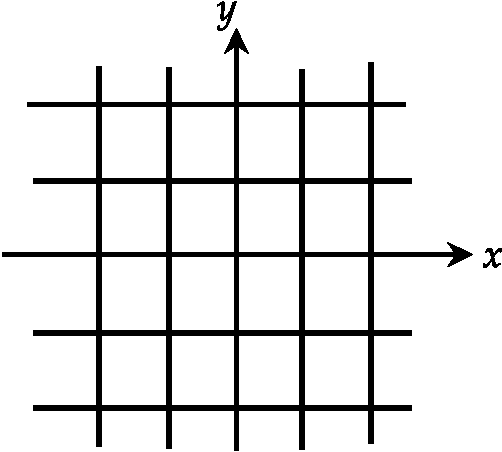
\includegraphics[height=3.5cm,width=4cm]{P -assignment-01}
	\end{figure}
	 \begin{tasks}(4)
		\task[\textbf{a.}]$\frac{1}{4}$
		\task[\textbf{b.}] $\frac{1}{8}$
		\task[\textbf{c.}]$\frac{1}{16}$
		\task[\textbf{d.}] $\frac{3}{16}$
	\end{tasks}
	\item If the density function of a random variable $X$ is $f(x)= \begin{cases}k x^{2}, & 1 \leq x \leq 5 \\ 0, & \text { otherwise }\end{cases}$
	Then the probability that the random variables assumes value between 2 to 4 is
	 \begin{tasks}(4)
		\task[\textbf{a.}]$\frac{15}{31}$
		\task[\textbf{b.}] $\frac{14}{31}$
		\task[\textbf{c.}]$\frac{17}{31}$
		\task[\textbf{d.}] $\frac{18}{31}$
	\end{tasks}
	\item For a continuous random variable $x$ probability distribution function
	$$
	f(x)= \begin{cases}c x^{2} & \text { for }|x| \leq 1 \\ 0 & \text { for }|x|>1\end{cases}
	$$
	Then the value of $c$ and $\operatorname{var}(x)$ are respectively
	 \begin{tasks}(4)
		\task[\textbf{a.}]$\frac{3}{2}, \frac{3}{5}$
		\task[\textbf{b.}] $\frac{3}{2}, \frac{5}{3}$
		\task[\textbf{c.}]$\frac{2}{3}, \frac{3}{5}$
		\task[\textbf{d.}] $\frac{2}{3}, \frac{5}{3}$
	\end{tasks}
	\item Consider the following two experiments:
	Experiment I: A pair of die is thrown 6 times. Let $P_{1}$ be the probability of getting a doublet on 5 throws (a doublet on a throw means same number on both die).
	
	Experiment II: A coin is tossed 6 times. Let $P_{2}$ be the probability of getting a head on 4 throws.
	The ratio of $P_{1}$ and $P_{2}$ is
	 \begin{tasks}(4)
		\task[\textbf{a.}]$\frac{1}{2^{5}}$
		\task[\textbf{b.}]$\frac{2}{3^{5}}$
		\task[\textbf{c.}]$\frac{1}{2^{6}}$
		\task[\textbf{d.}]$\frac{2}{3^{6}}$
	\end{tasks}
	
	
	
	
	
	
	
	
	
	
	
	
	
	
	
	
	
	
	
	
	
	
	
	
	
	
	
	
	
	
	
	
	
	
	
	
	
	
\end{enumerate}